        \subsection{Vymezení pojmů}
        Pro lepší porozumění textu této práce je potřeba definovat pojmy replikace,
        synchronizace a verzování, včetně popisu toho, jak jsou dané pojmy chápány v
        produktech ArcGIS. Je vhodné upozornit, že výše zmíněné procesy jsou v
        literatuře často chápány lehce odlišně. Některé zdroje pojmy replikace a
        synchronizace rozlišují, jiné je naopak považují za synonyma. 

        Všechny dotyčné pojmy úzce souvisí se zálohováním dat, tedy kopírovaním dat
        mezi dvěmi a více uložišti. To, co tyto pojmy spojuje, je totiž vždy, v nějaké
        míře, zabránění ztrátě dat, ať už chybou či fyzickým poškozením disku. Dané
        pojmy se poté liší například konkrétním způsobem provedení zálohy, či přesným
        důvodem kopírování dat. 

        Z mého pohledu je synchronizace nadmnožinou replikace. V případě, že existují
        dva datové zdroje a v jeden okamžik se rozhodneme, že chceme tyto dvě složky
        sjednotit, poté je možno mluvit o synchronizaci souborů či datových složek.
        Soubor, který se podle názvu nachází ve složce A a zároveň se nenachází ve
        složce B, se jednoduše zkopíruje do složky A. U souborů se stejným názvem, se
        dále porovnává čas posledního zápisu, velikost nebo obsah souboru. Poté je
        soubor se starším datem, resp. menší velikostí, přepsán tím novějším, resp.
        větším. Synchronizací se tedy dá proces označit v okamžiku, kdy existují
        nejméně dva datové zdroje a smyslem synchronizace je porovnat tato uložiště a
        dostat je do stejného stavu. To může například přispět snazší spolupráci více
        uživatelů nad stejnými daty nebo uživateli, který pracuje na více počítačích.
        %parametr H říká že to bude přímo na tom místě kde je v textu...více http://en.wikibooks.org/wiki/LaTeX/Floats,_Figures_and_Captions
          \begin{figure}[H]
            \centering
            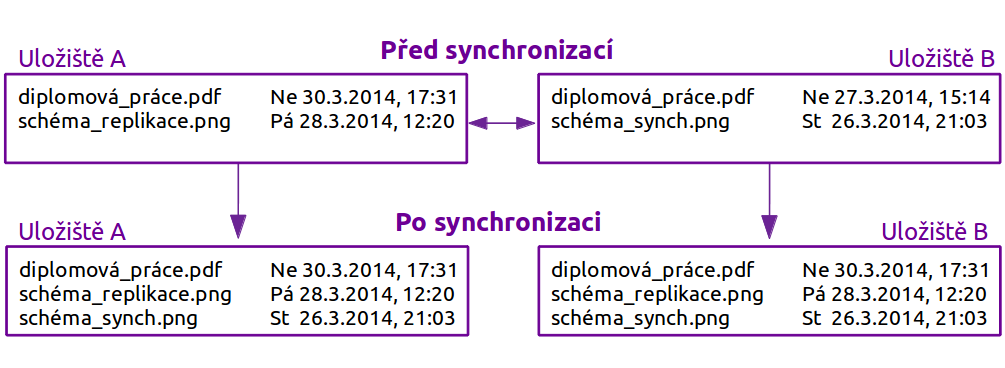
\includegraphics[scale=1]{../../../grafy/obr/schema_synchronizace_vetsi.png}
            \caption {Příklad obousměrné synchronizace dat mezi dvěmi datovými uložišti}
          \end{figure}
          \begin{figure}[H]
            \centering
            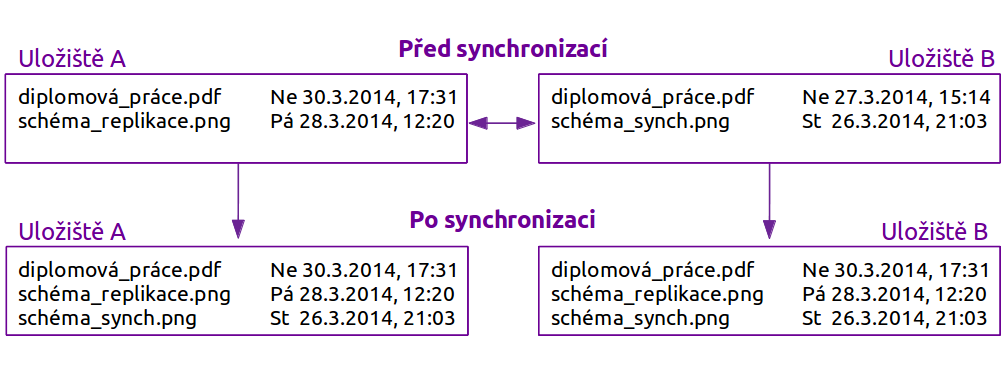
\includegraphics[scale=1]{../../../grafy/obr/schema_synchronizace_tence.png}
            \caption {Příklad obousměrné synchronizace dat mezi dvěmi datovými uložišti}
          \end{figure}
        Replikace naopak, podle mého názoru, začíná s daty existujícími pouze na jednom
        uložišti. Často je tento proces používán právě ve spojitosti s databázemi, kdy
        je kopie dat (také replika) tvořena z důvodu snížení zátěže serveru, či ochraně
        dat. V případě, že je tato kopie již vytvořena, je poté možno mluvit i o
        synchronizaci dat, protože replika průběžně kontroluje, zda na hlavním serveru
        nedošlo ke změně, a pokud ano, dané změny zkopíruje.

        Oba procesy je možno použít jednostranně, tedy kopírovat data pouze z jednoho
        uložiště na druhé a nikolik opačně, nebo oboustraně, kdy se datové zdroje
        kopírují navzájem mezi sebou.

        Specifickým způsobem zálohy dat je verzování, kdy se data na záložním datovém
        uložišti nepřepisují, ale systematicky ukládající v takzvaných verzích tak, aby
        se uživatel mohl snadno kdykoliv vrátit k předchozím stavům souborů. Smyslem
        verzování je zachovat všechny zvolené stavy práce, čímž se verzování liší od
        zálohování, kde stačí mít aktuální kopii daných dat. To, co je zde popsáno jako
        verzování, se v produktech ArcGIS nazývá archivování dat \citep{Law2008}. 

        Verzování může probíhat ručně, poloautomatizovaně či plně automatizovaně díky
        speciálním nástrojům pro správu verzí. Oblíbeným verzovací systémem
        programátorů je GIT\footnote{Více na http://git-scm.com/}, open-source nástroj
        pro správu verzí, který pomáhá při práci s malými i velkými projekty a
        podporuje týmovou spolupráci. Umožňuje vrátit jednotlivé soubory nebo celý
        projekt do předchozího stavu, porovnávat změny provedené v průběhu času,
        zjistit, kdo naposledy upravil něco, co nyní možná způsobuje problémy, kdo
        vložil jakou verzi a mnoho dalšího \citep{Chacon2009}. GIT je vhodný zejména
        pro textové soubory, protože dokáže analyzovat části textu, či programového
        kódu a zvýraznit části, které se změnily.
        
          \begin{figure}[H]
            \centering
            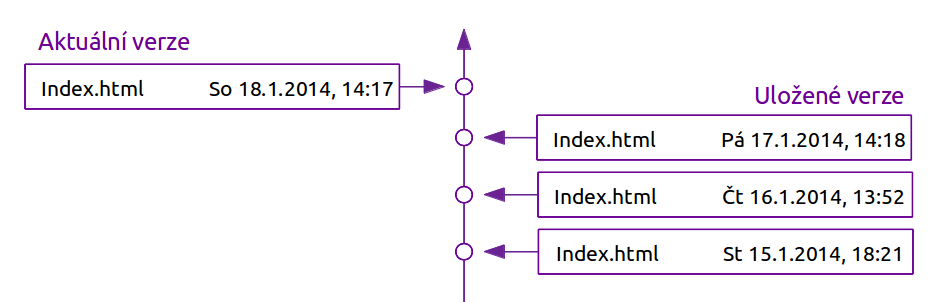
\includegraphics[scale=1]{../../../grafy/obr/schema_verzovani_tence.png}
            \caption {Příklad verzování souboru}
          \end{figure}

        Samotná databáze verzování dat neumožňuje. Nejsnazším způsobem, jak získat
        verzi dat, je dump, tedy export databáze do souboru. V MS SQL Serveru je tento
        prces nazýván Snapshot, tedy snímek databáze nebo také snímková replikace.
        Takový soubor se poté může verzovat podobným způsobem jako jakýkoliv jiný
        binární soubor typu shapefile. A to samé platí i pokud v databázi ukládáme
        geodata. 

        Proto byl vytvořen verzovací systém také pro prostorová data, který vychází ze
        systému gitu a nese název GeoGIT. Umožňuje uživatelům zachovávat změny v
        souborech shapefile, SpatialLite a z databáze PostGIS (PostgreSQL). Umožňuje,
        tak jako git, uchovávat historii prostorových dat, či vrátit se k předchozí
        verzi. 

        Verzování může být chápáno také jako vytvoření pracovní verze. V případě, že
        programový kód či data jsou plno funkční či aktuální, ale je potřeba je
        testovit či jinak měnit, pak je vhodné vytvořit tzn. pracovní verzi, aby
        nedošlo k poškození té správné. Pracovní verze je kopie aktuálního stavu, na
        které je možno pracovat a zkoušet. V případě, že práce nedopadne podle přestav,
        je možno změny zahodit, pokud je tomu naopak, je možno pracovní verzi sjednotit
        s platnou verzí. Tento způsob verzování umožňuje GIT i GeoGIT a takto chápe
        pojem verzování i společnosti Esri.

          \begin{figure}[H]
            \centering
            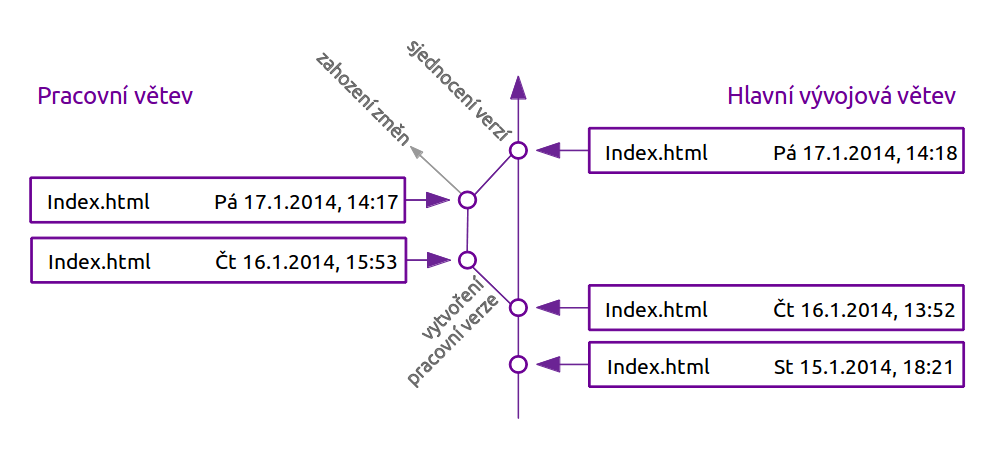
\includegraphics[scale=1]{../../../grafy/obr/schema_verzovani_branch_vetsi.png}
            \caption {Příklad verzování souboru s použitím pracovní větve}
          \end{figure}

        

